\documentclass[12pt,addpoints]{repaso}
\grado{2}
\nivel{Primaria}
\cicloescolar{2024-2025}
\materia{Matemáticas}
\unidad{1}
\title{Practica la Unidad}
\aprendizajes{\scriptsize%
\item Expresa oralmente la sucesión numérica hasta cuatro cifras, en español y hasta donde sea posible, en su lengua materna, de manera ascendente y descendente a partir de un número natural dado.\\[-1.8em]
\item Representa, con apoyo de material concreto y modelos gráficos, fracciones: medios, cuartos, octavos, dieciseisavos, para expresar el resultado de mediciones y repartos en situaciones vinculadas a su contexto.\\[-1.8em]
\item Resuelve situaciones problemáticas vinculadas a su contexto que implican sumas, restas, multiplicación y división de números naturales de hasta tres cifras utilizando el algoritmo convencional y que impliquen, medición, estimación y comparación, de longitudes, masas y capacidades, con el uso del metro, kilogramo, litro y medios y cuartos de estas unidades; en el caso de la longitud, el decímetro y centímetro.\\[-1.8em]
   }
\author{Melchor Pinto, JC}
\begin{document}
\INFO
% \begin{multicols}{2}
\tableofcontents
% \end{multicols}
\begin{questions}\large
	\addcontentsline{toc}{section}{Unidad 1}
	\section*{Unidad 1}

	\addcontentsline{toc}{subsection}{Conteo de números}
	\subsection*{Conteo de números}

	\questionboxed[5]{Escribe sobre la línea la cantidad de puntos {\color{red} rojos} que aparecen en cada figura:

		\begin{multicols}{5}
			\begin{parts}
				\part 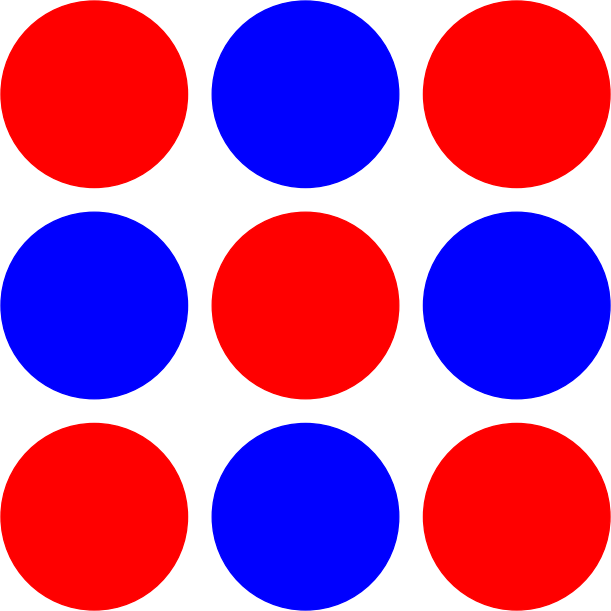
\includegraphics[width=45px]{../images/imagen_puntos01.png} \fillin[ 5][1.5cm]
				\part 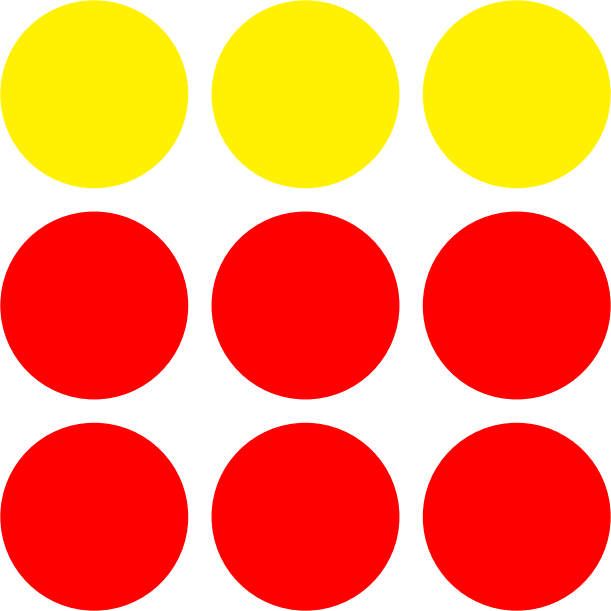
\includegraphics[width=45px]{../images/imagen_puntos05.png} \fillin[ 6][1.5cm]
				\part 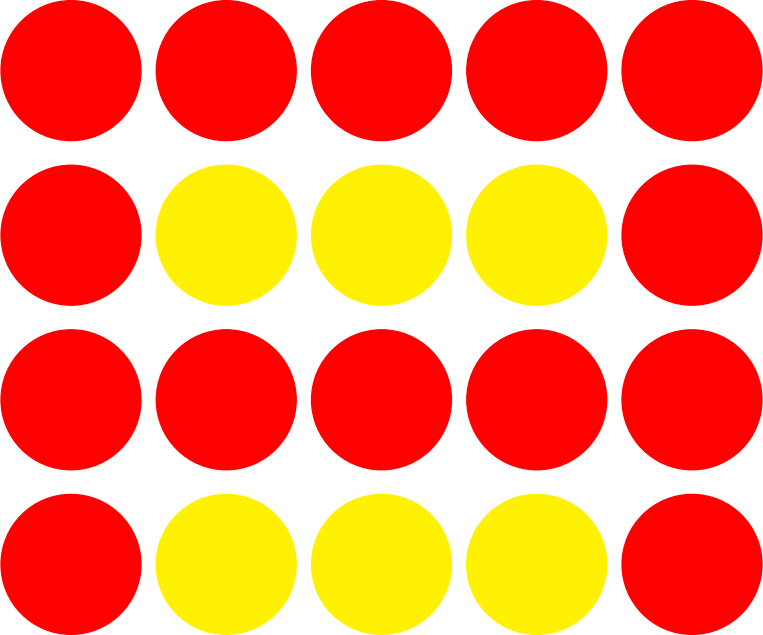
\includegraphics[width=45px]{../images/imagen_puntos09.png} \fillin[14][1.5cm]
				\part 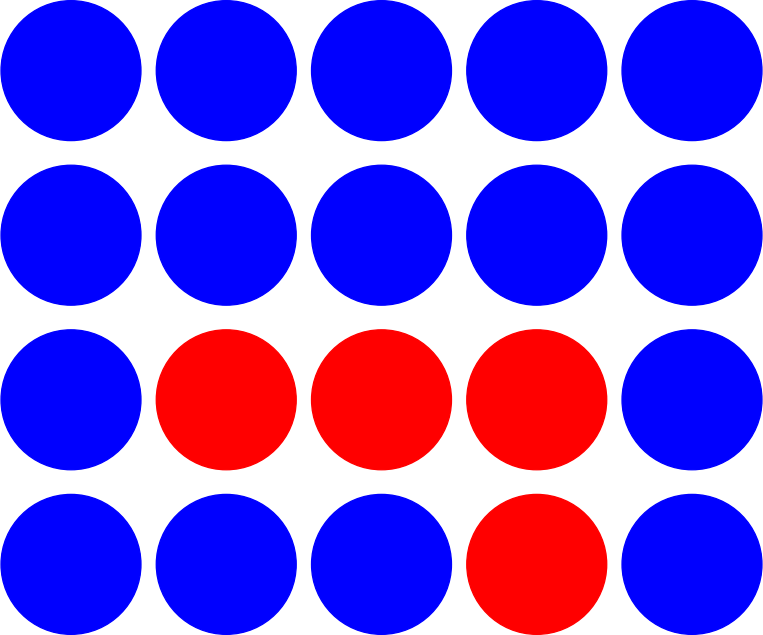
\includegraphics[width=45px]{../images/imagen_puntos13.png} \fillin[ 4][1.5cm]
				\part 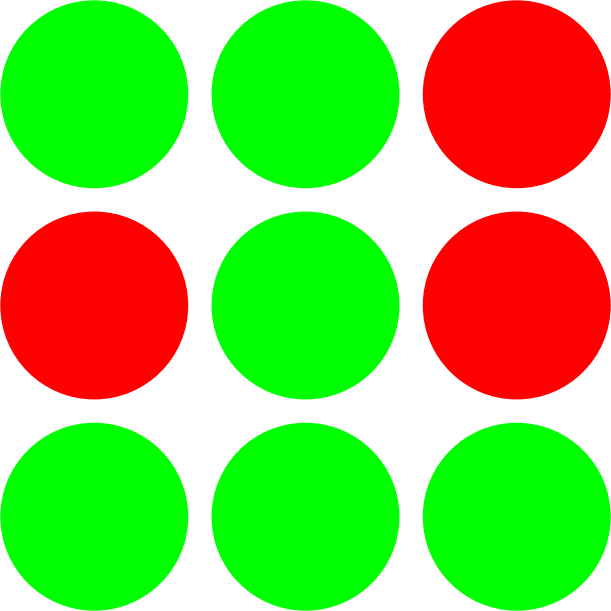
\includegraphics[width=45px]{../images/imagen_puntos02.png} \fillin[ 3][1.5cm]
				\part 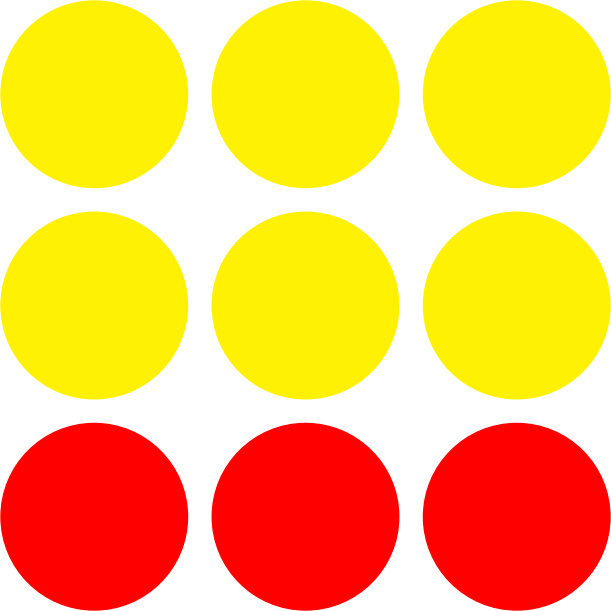
\includegraphics[width=45px]{../images/imagen_puntos06.png} \fillin[ 3][1.5cm]
				\part 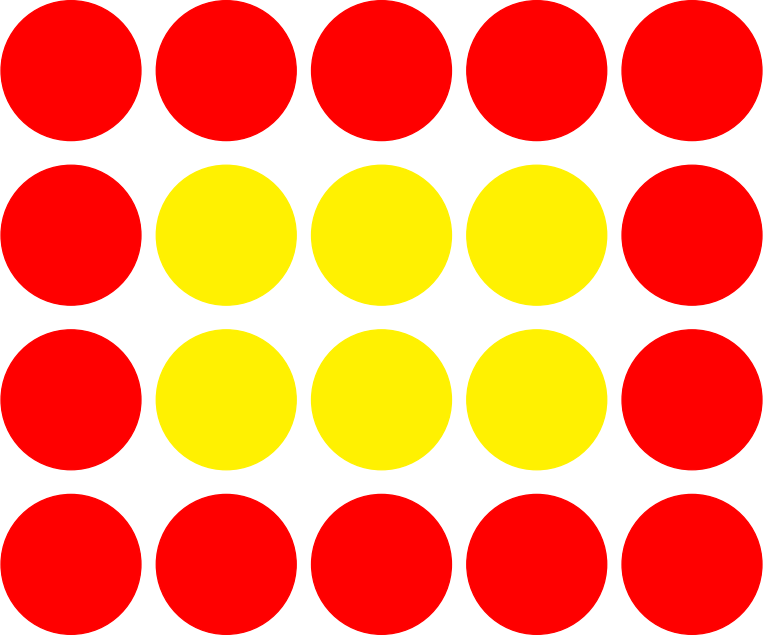
\includegraphics[width=45px]{../images/imagen_puntos10.png} \fillin[14][1.5cm]
				\part 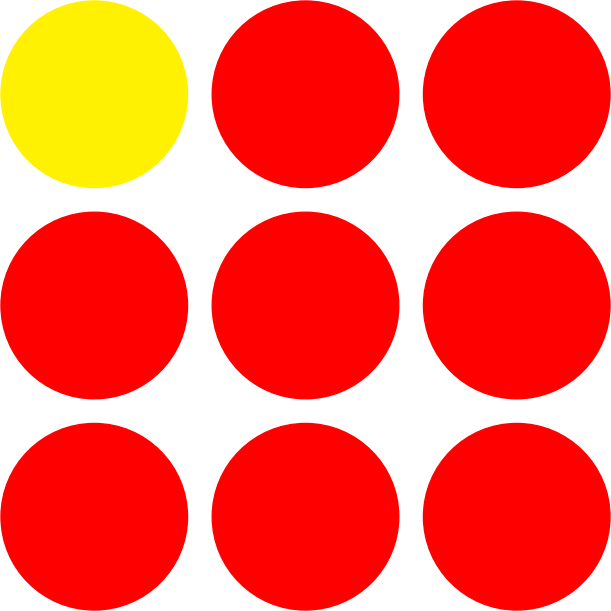
\includegraphics[width=45px]{../images/imagen_puntos07.png} \fillin[ 8][1.5cm]
				\part 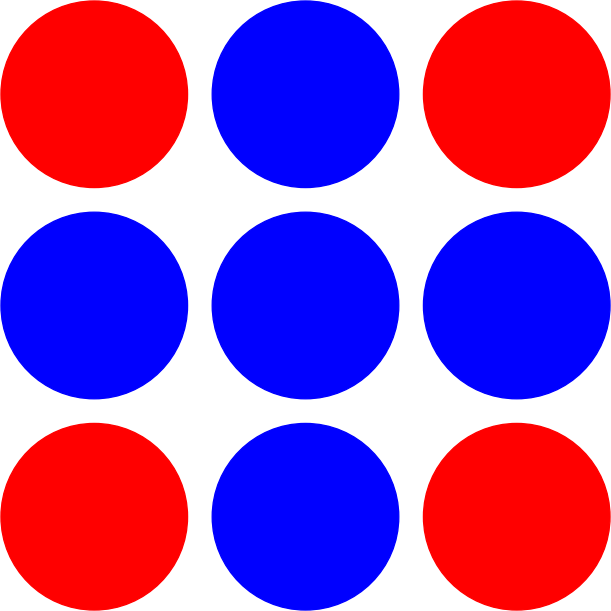
\includegraphics[width=45px]{../images/imagen_puntos03.png} \fillin[ 4][1.5cm]
				\part 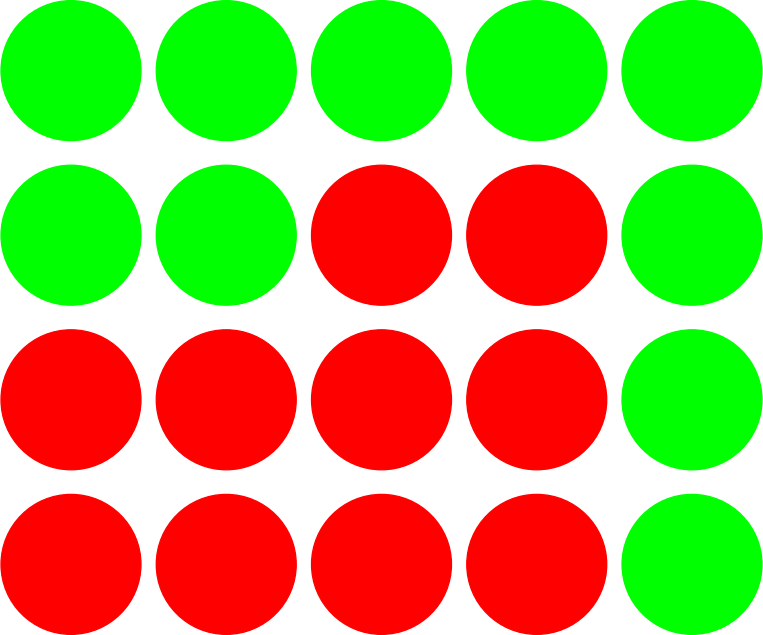
\includegraphics[width=45px]{../images/imagen_puntos14.png} \fillin[10][1.5cm]
				\part 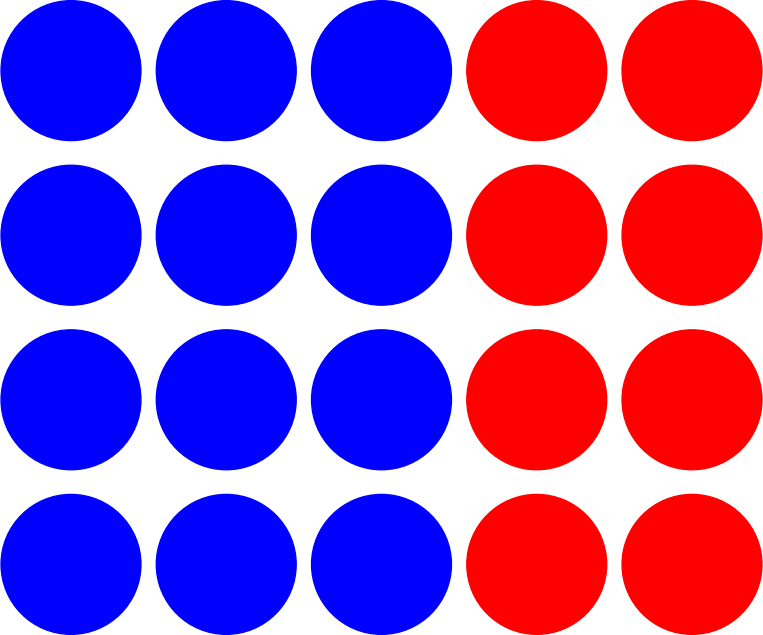
\includegraphics[width=45px]{../images/imagen_puntos11.png} \fillin[ 8][1.5cm]
				\part 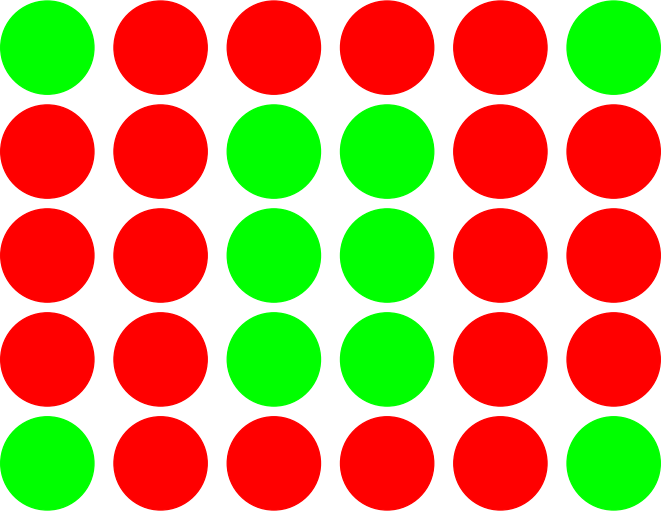
\includegraphics[width=45px]{../images/imagen_puntos15.png} \fillin[20][1.5cm]
				% \part 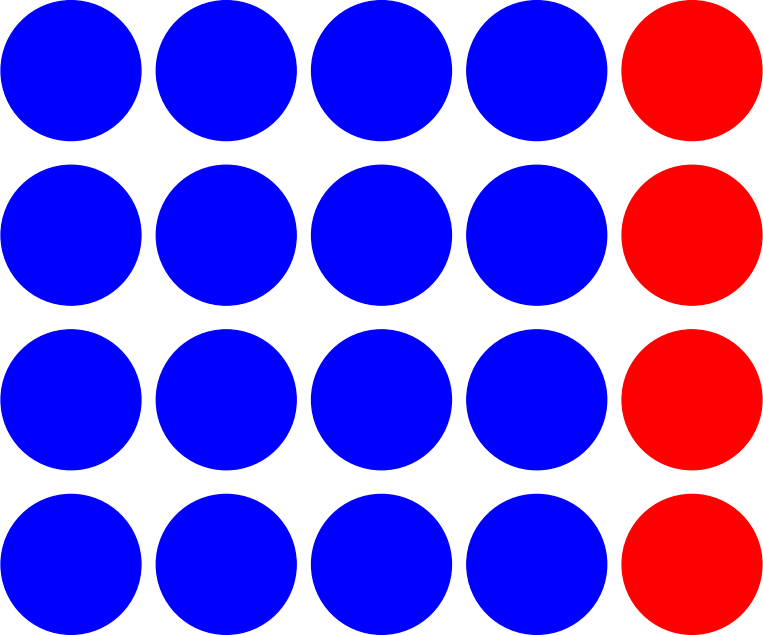
\includegraphics[width=45px]{../images/imagen_puntos12.png} \fillin[ 4][1.5cm] 
				\part 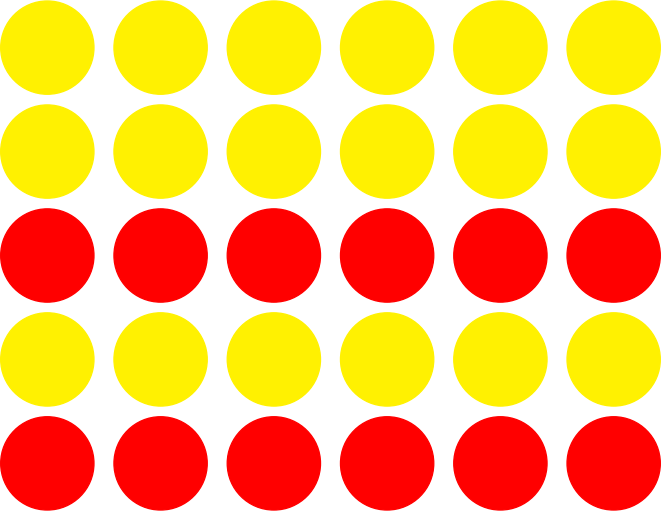
\includegraphics[width=45px]{../images/imagen_puntos16.png} \fillin[10][1.5cm]
				\part 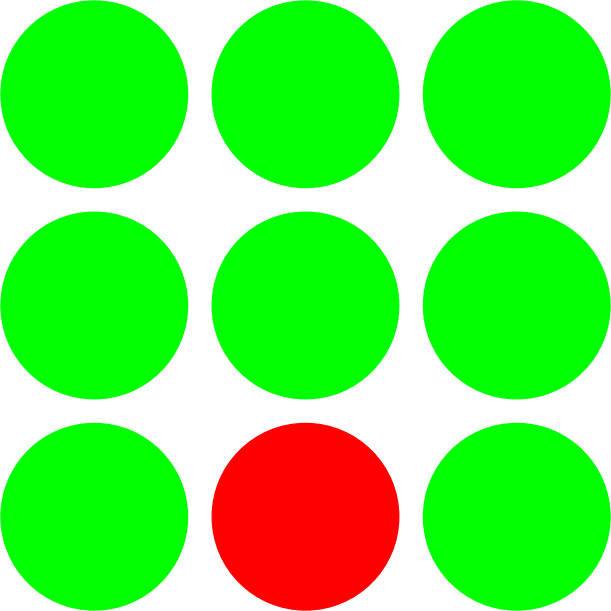
\includegraphics[width=45px]{../images/imagen_puntos04.png} \fillin[ 1][1.5cm]
				\part 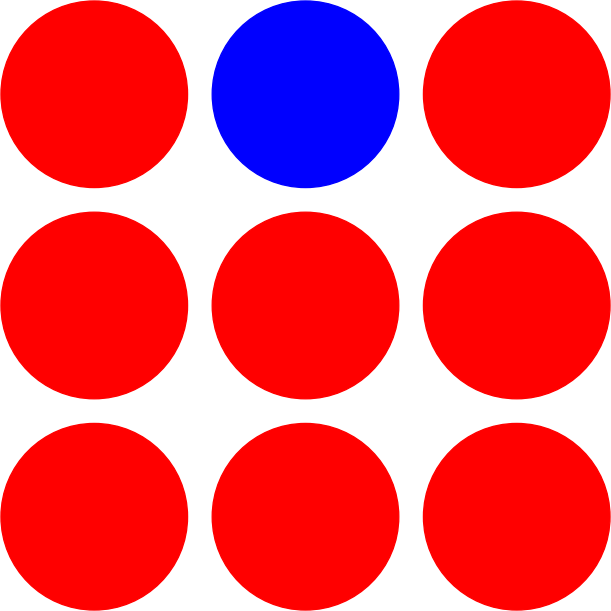
\includegraphics[width=45px]{../images/imagen_puntos08.png} \fillin[ 8][1.5cm]
			\end{parts}
		\end{multicols}
	}

	\questionboxed[5]{Escribe sobre la línea la cantidad de puntos {\color{red} rojos} que aparecen en cada figura:

		\begin{multicols}{5}
			\begin{parts}
				\part 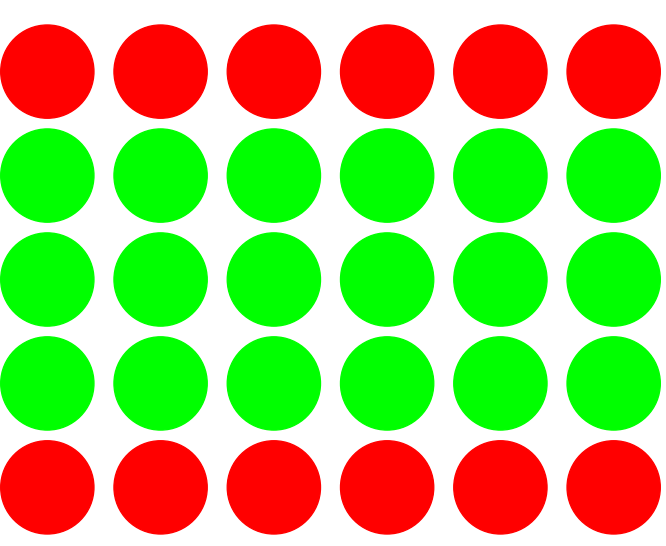
\includegraphics[width=45px]{../images/imagen_puntos17.png} \fillin[12][1.5cm]
				\part 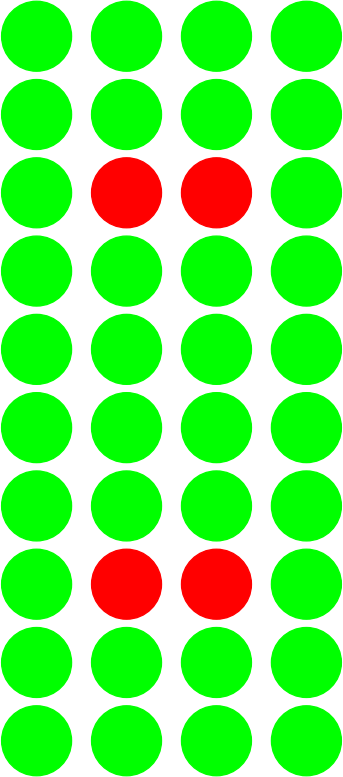
\includegraphics[width=45px]{../images/imagen_puntos25.png} \fillin[ 4][1.5cm]
				\part 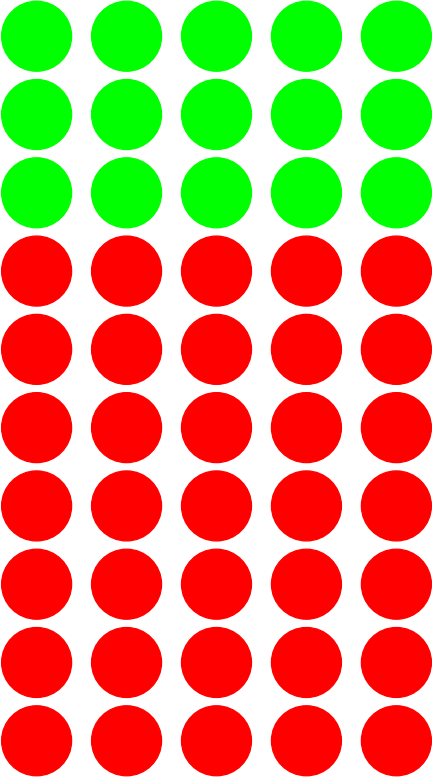
\includegraphics[width=45px]{../images/imagen_puntos29.png} \fillin[35][1.5cm]
				\part 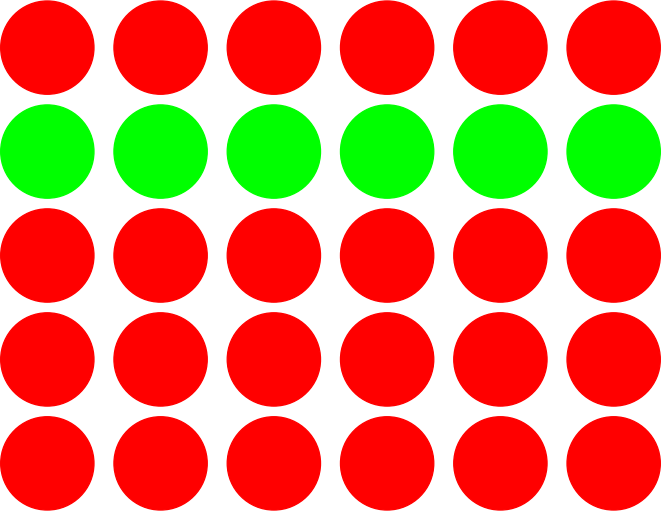
\includegraphics[width=45px]{../images/imagen_puntos21.png} \fillin[24][1.5cm]
				\part 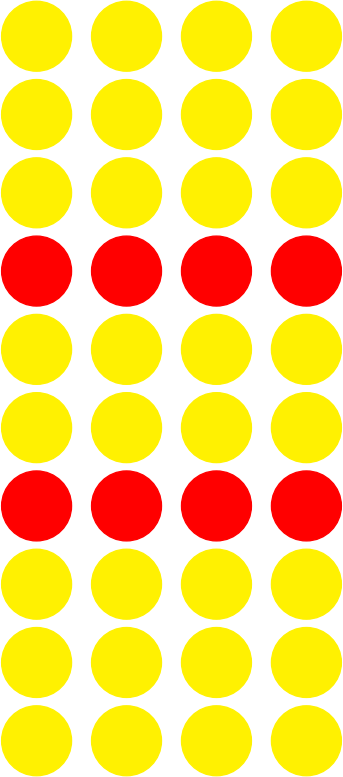
\includegraphics[width=45px]{../images/imagen_puntos22.png} \fillin[ 8][1.5cm]
				\part 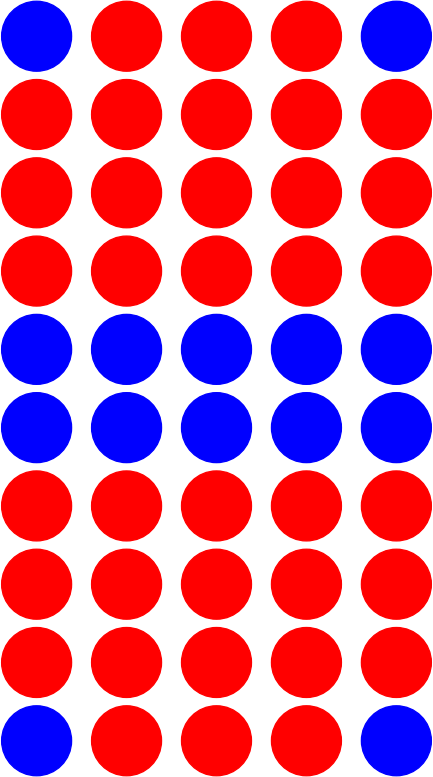
\includegraphics[width=45px]{../images/imagen_puntos30.png} \fillin[36][1.5cm]
				\part 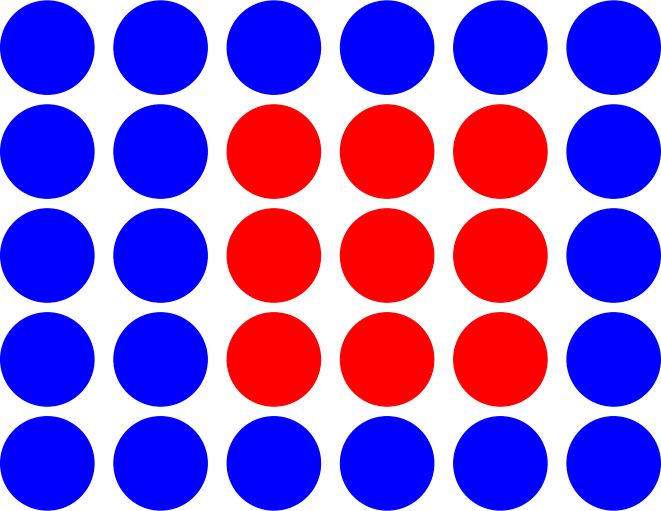
\includegraphics[width=45px]{../images/imagen_puntos18.png} \fillin[ 9][1.5cm]
				\part 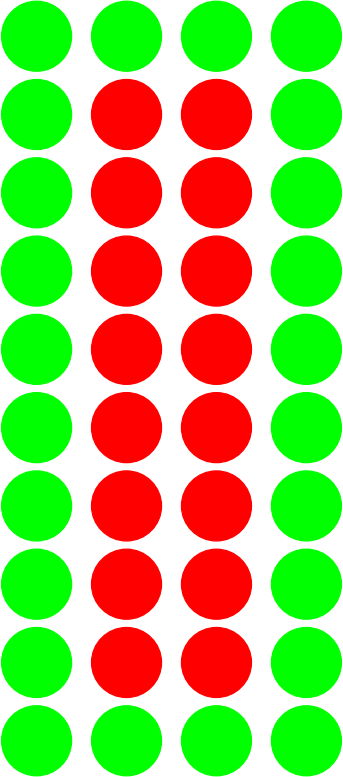
\includegraphics[width=45px]{../images/imagen_puntos26.png} \fillin[16][1.5cm]
				\part 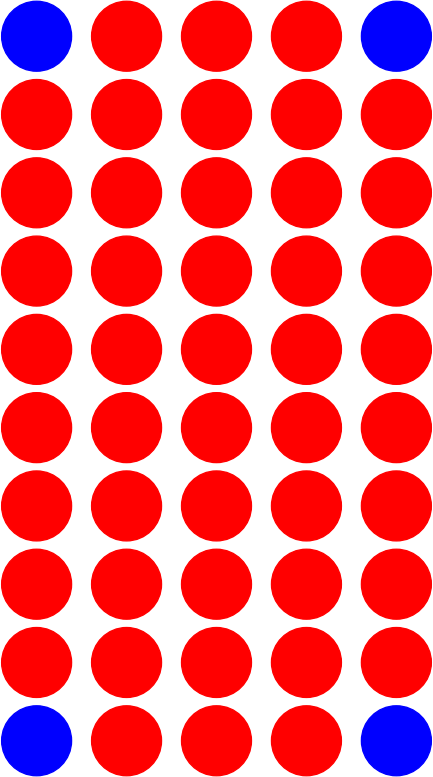
\includegraphics[width=45px]{../images/imagen_puntos31.png} \fillin[46][1.5cm]
				\part 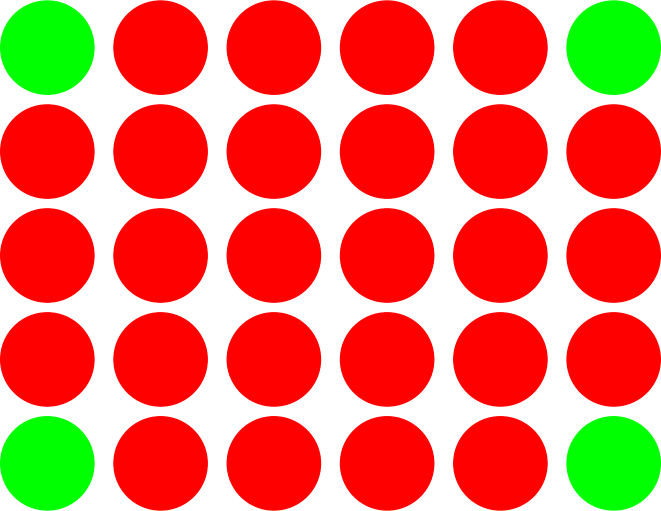
\includegraphics[width=45px]{../images/imagen_puntos19.png} \fillin[26][1.5cm]
				\part 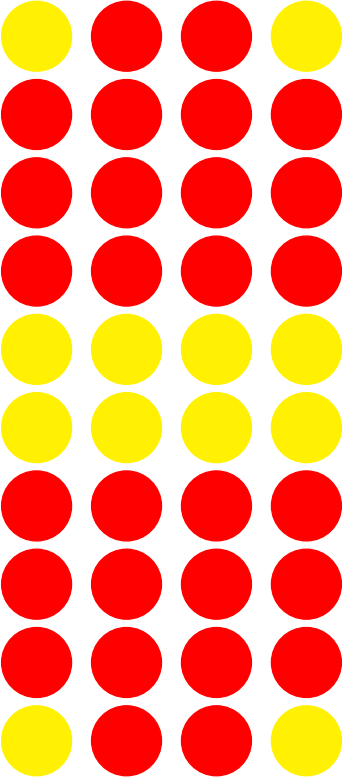
\includegraphics[width=45px]{../images/imagen_puntos23.png} \fillin[28][1.5cm]
				\part 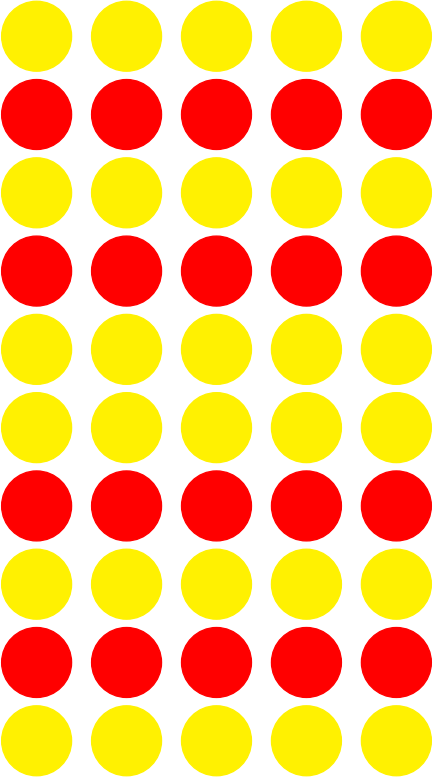
\includegraphics[width=45px]{../images/imagen_puntos28.png} \fillin[20][1.5cm]
				% \part 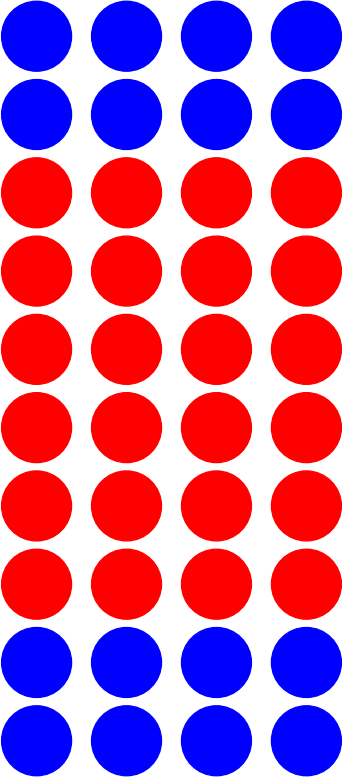
\includegraphics[width=45px]{../images/imagen_puntos27.png} \fillin[24][1.5cm] 
				\part 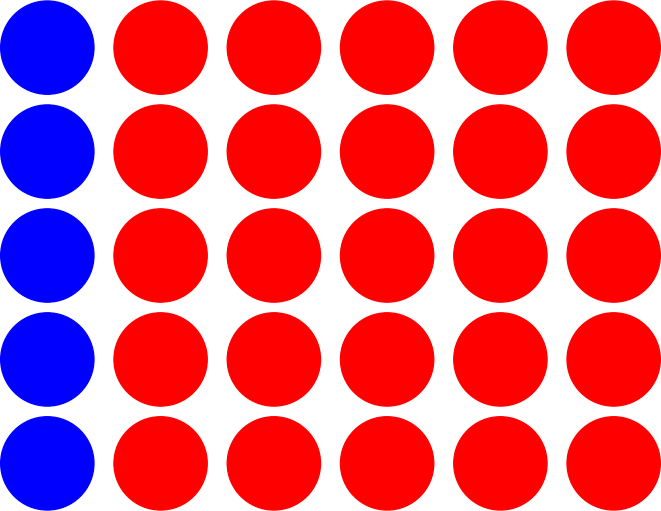
\includegraphics[width=45px]{../images/imagen_puntos20.png} \fillin[25][1.5cm]
				\part 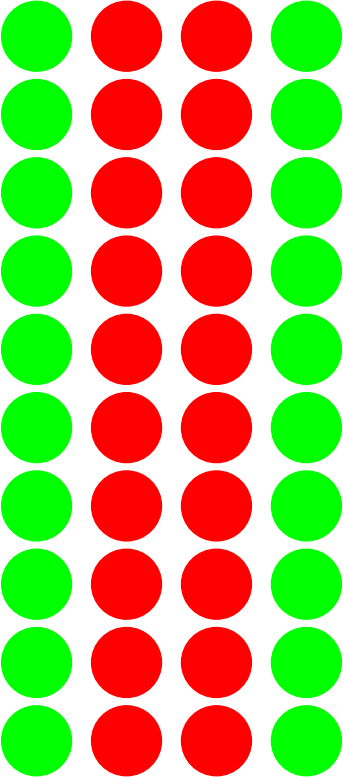
\includegraphics[width=45px]{../images/imagen_puntos24.png} \fillin[20][1.5cm]
				\part 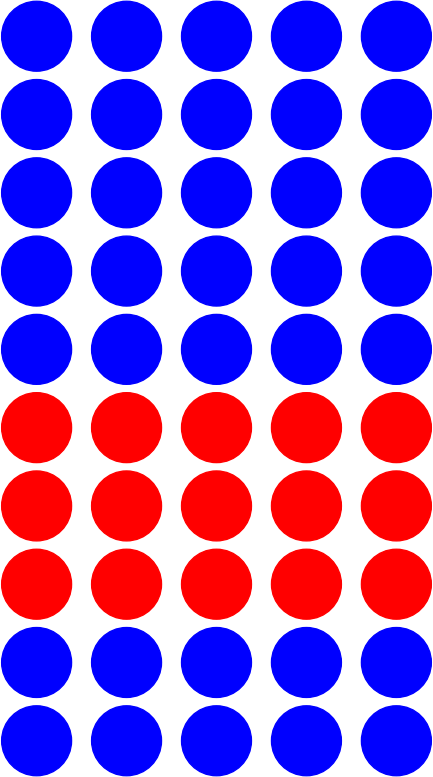
\includegraphics[width=45px]{../images/imagen_puntos32.png} \fillin[15][1.5cm]
			\end{parts}
		\end{multicols}
	}


	\addcontentsline{toc}{subsection}{Escritura de cantidades}
	\subsection*{Escritura de cantidades}


	\questionboxed[5]{Escribe sobre la línea los siguientes números:

		\begin{multicols}{3}
			\begin{parts}
				\part \fillin[ 2][0.5cm] Dos
				\part \fillin[19][0.5cm] Diecinueve
				\part \fillin[32][0.5cm] Treinta y dos
				\part \fillin[16][0.5cm] Dieciséis
				\part \fillin[21][0.5cm] Veintiuno
				\part \fillin[67][0.5cm] Sesenta y siete
				\part \fillin[51][0.5cm] Cincuenta y uno


				\part \fillin[ 5][0.5cm] Cinco
				\part \fillin[43][0.5cm] Cuarenta y tres
				\part \fillin[11][0.5cm] Once
				\part \fillin[18][0.5cm] Dieciocho
				\part \fillin[22][0.5cm] Veintidos
				\part \fillin[89][0.5cm] Ochenta y nueve
				% \part \fillin[][0.5cm] Veintinueve
				\part \fillin[76][0.5cm] Setenta y seis

				\part \fillin[ 9][0.5cm] Nueve
				\part \fillin[13][0.5cm] Trece
				\part \fillin[15][0.5cm] Quince
				\part \fillin[12][0.5cm] Doce
				\part \fillin[27][0.5cm] Veintisiete
				\part \fillin[60][0.5cm] Sesenta
				\part \fillin[75][0.5cm] Setenta y cinco
			\end{parts}
		\end{multicols}
	}


	\addcontentsline{toc}{subsection}{Recta numérica}
	\subsection*{Recta numérica}

	\questionboxed[5]{Escribe en el recuadro el número que representa el punto en la recta numérica de cada imagen:

		\begin{multicols}{2}
			\begin{parts}
				\part 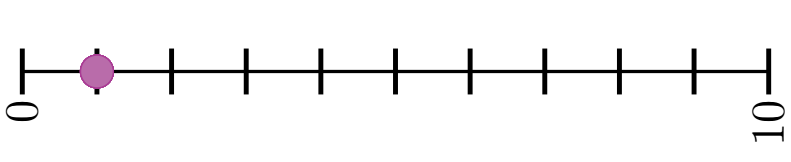
\includegraphics[width=180px]{../images/recta_num_1.png}   \hfill \fillin[ 1][1cm]
				\part 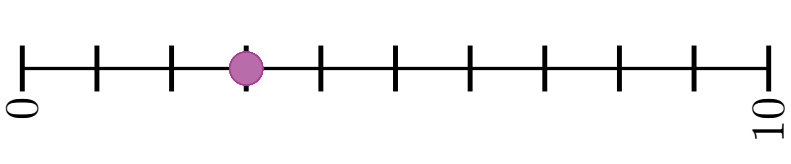
\includegraphics[width=180px]{../images/recta_num_3.png}   \hfill \fillin[ 3][1cm]
				\part 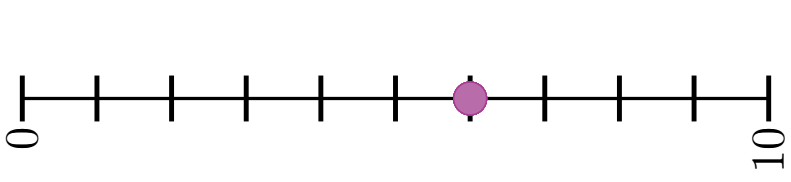
\includegraphics[width=180px]{../images/recta_num_6.png}   \hfill \fillin[ 6][1cm]
				\part 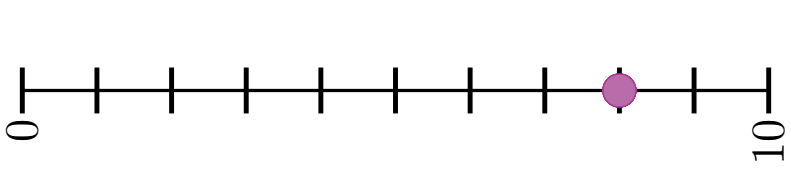
\includegraphics[width=180px]{../images/recta_num_8.png}   \hfill \fillin[ 8][1cm]
				\part 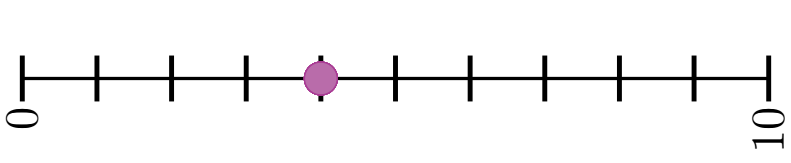
\includegraphics[width=180px]{../images/recta_num_4.png}   \hfill \fillin[ 4][1cm]
				\part 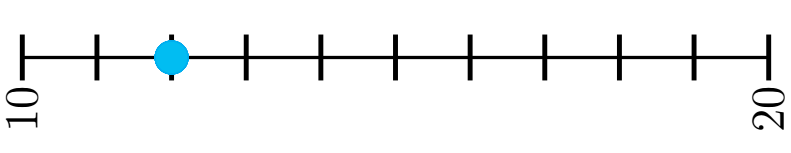
\includegraphics[width=180px]{../images/recta_num_12.png}  \hfill \fillin[12][1cm]
				\part 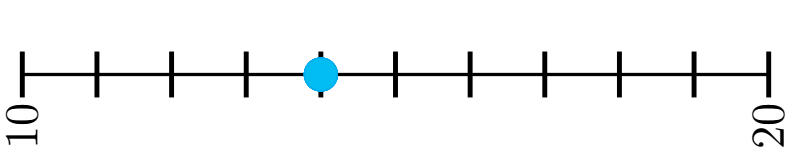
\includegraphics[width=180px]{../images/recta_num_14.png}  \hfill \fillin[14][1cm]
				\part 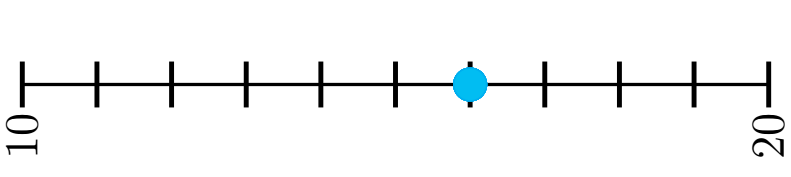
\includegraphics[width=180px]{../images/recta_num_16.png}  \hfill \fillin[16][1cm]
				\part 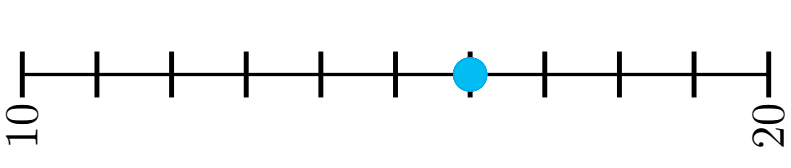
\includegraphics[width=180px]{../images/recta_num_17.png}  \hfill \fillin[17][1cm]
				\part 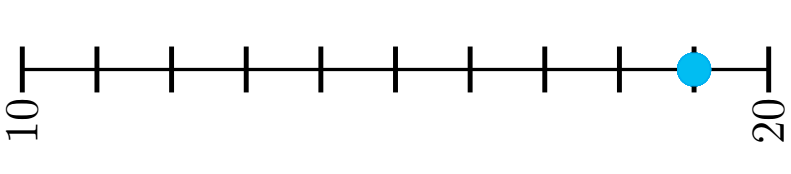
\includegraphics[width=180px]{../images/recta_num_19.png}  \hfill \fillin[19][1cm]
			\end{parts}
		\end{multicols}
	}

	\questionboxed[5]{Escribe en el recuadro el número que representa el punto en la recta numérica de cada imagen:

		\begin{multicols}{2}
			\begin{parts}
				\part 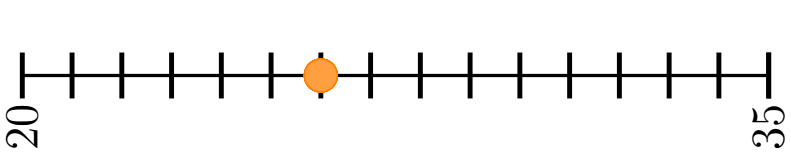
\includegraphics[width=180px]{../images/recta_num_26.png}   \hfill \fillin[26][1cm]
				\part 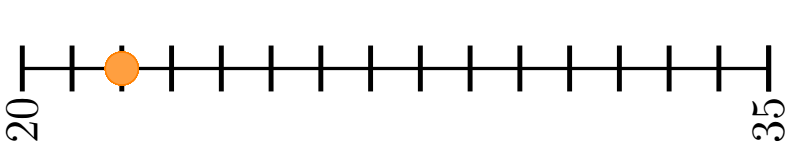
\includegraphics[width=180px]{../images/recta_num_21.png}   \hfill \fillin[21][1cm]
				\part 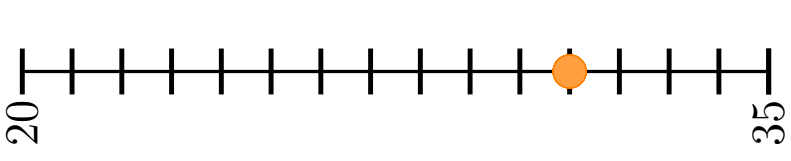
\includegraphics[width=180px]{../images/recta_num_31.png}   \hfill \fillin[31][1cm]
				\part 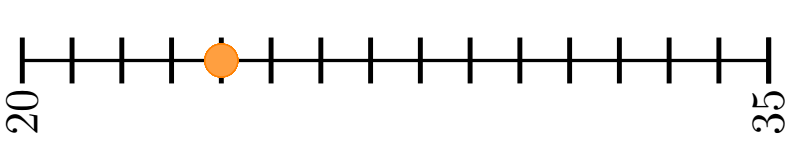
\includegraphics[width=180px]{../images/recta_num_24.png}   \hfill \fillin[24][1cm]
				\part 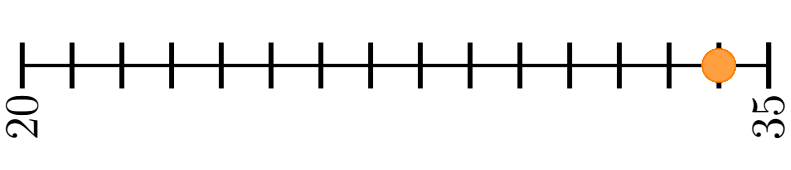
\includegraphics[width=180px]{../images/recta_num_34.png}   \hfill \fillin[34][1cm]
				\part 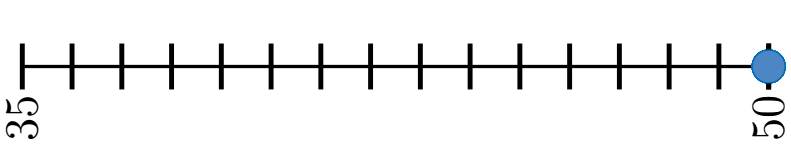
\includegraphics[width=180px]{../images/recta_num_50.png}   \hfill \fillin[50][1cm]
				\part 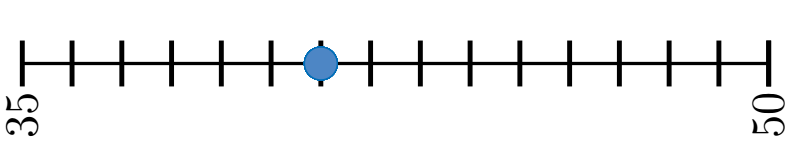
\includegraphics[width=180px]{../images/recta_num_41.png}   \hfill \fillin[41][1cm]
				\part 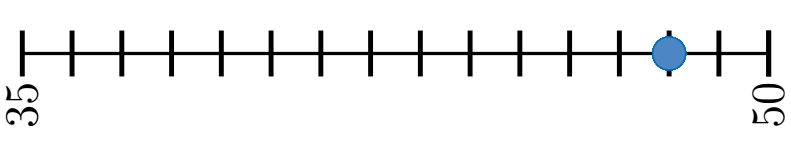
\includegraphics[width=180px]{../images/recta_num_48.png}   \hfill \fillin[48][1cm]
				\part \includegraphics[width=180px]{../images/recta_num_36.png}   \hfill \fillin[36][1cm]
				\part \includegraphics[width=180px]{../images/recta_num_39.png}   \hfill \fillin[39][1cm]
			\end{parts}
		\end{multicols}
	}

	\addcontentsline{toc}{subsection}{Sistema decimal}
	\subsection*{Sistema decimal}

	\questionboxed[5]{Señala la opción que responda correctamente a cada una de las siguientes preguntas:

		\begin{multicols}{2}
			\begin{parts}
				\part ¿Qué lugar ocupa el 8 en 6418?     \fillin[C][0.5cm]
				\part ¿Qué lugar ocupa el 4 en 206418?   \fillin[A][0.5cm]
				\part ¿Qué lugar ocupa el 6 en 87264?    \fillin[B][0.5cm]
				% \part ¿Qué lugar ocupa el 4 en 1684?     \fillin[C][0.5cm]
				% \part ¿Qué lugar ocupa el 1 en 6138?     \fillin[A][0.5cm]
				% \part ¿Qué lugar ocupa el 4 en 198114?   \fillin[C][0.5cm]
				\part ¿Qué lugar ocupa el 8 en 149778?   \fillin[C][0.5cm]
				\part ¿Qué lugar ocupa el 7 en 46878?    \fillin[B][0.5cm]
			\end{parts}

			\columnbreak%

			\begin{choices}\Large
				\choice {\color{red}centenas.}
				\choice {\color{blue}decenas.}
				\choice {\color{Goldenrod!65!black}unidades.}
			\end{choices}
		\end{multicols}
	}

	\questionboxed[6]{Escribe la notación desarrollada de cada uno de los siguientes números:

		\begin{multicols}{3}
			\begin{parts}
				\part $28=$ \fillin[$20+8$][1in]
				\part $84=$ \fillin[$80+4$][1in]
				\part $77=$ \fillin[$70+7$][1in]
				\part $936 =$ \fillin[$900+30+6$][1in]

				\part $11 =$ \fillin[$10+1$][1in]
				\part $48 =$ \fillin[$40+8$][1in]
				\part $96=$ \fillin[$90+6$][1in]
				\part $215 =$ \fillin[$200+10+5$][1in]

				\part $39=$ \fillin[$30+9$][1in]
				\part $57 =$ \fillin[$50+7$][1in]
				\part $79=$ \fillin[$70+9$][1in]
				\part $105 =$ \fillin[$100+5$][1in]
			\end{parts}
		\end{multicols}
	}
\end{questions}
\end{document}